\begin{frame}{Vector Similarity Search with FAISS}

\begin{columns}[T]
  \begin{column}{0.55\textwidth}
    \begin{itemize}
        \item Used \textbf{Facebook AI Similarity Search (FAISS)} library which performs L2 (Euclidean) distance search in embedding space
        \item Index built with:
          \begin{itemize}
            \item 5160 book embeddings (\( \vec{v} \in \mathbb{R}^{384} \))
            \item Exact search (IndexFlatL2)
          \end{itemize}
        \item At runtime:
          \begin{itemize}
            \item User query is embedded
            \item Top-k nearest neighbors retrieved
            \item Results shown in UI
            \item \textbf{Fully local}, fast search
          \end{itemize}
        \item Example Queries
          \begin{itemize}
            \item "Instead of 'fantasy dragons', user can type 'books about magical creatures'"
            \item "'philosophical science fiction' finds books exploring deep questions"
            \item "'unreliable narrator mystery' - semantic understanding of literary techniques"
          \end{itemize}
    \end{itemize}
  \end{column}

  \begin{column}{0.40\textwidth}
    \centering
    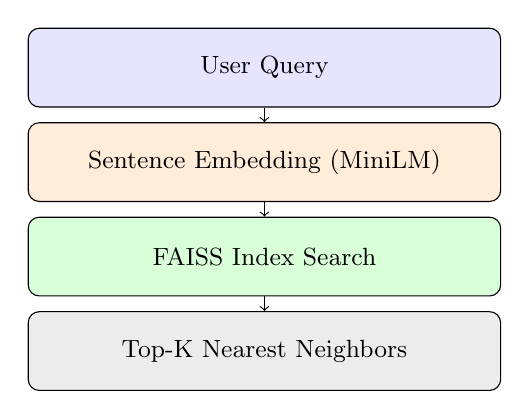
\begin{tikzpicture}[node distance=1.2cm, every node/.style={font=\small}]
        \node (query) [draw, rounded corners, minimum width=6cm, minimum height=1cm, fill=blue!10] {User Query};

        \node (embed) [below of=query, draw, rounded corners, minimum width=6cm, minimum height=1cm, fill=orange!15] {Sentence Embedding (MiniLM)};

        \node (faiss) [below of=embed, draw, rounded corners, minimum width=6cm, minimum height=1cm, fill=green!15] {FAISS Index Search};

        \node (results) [below of=faiss, draw, rounded corners, minimum width=6cm, minimum height=1cm, fill=gray!15] {Top-K Nearest Neighbors};

        \draw[->] (query) -- (embed);
        \draw[->] (embed) -- (faiss);
        \draw[->] (faiss) -- (results);
    \end{tikzpicture}
  \end{column}
\end{columns}

\end{frame}

\note{
  \begin{columns}[T]
    \begin{column}{0.49\textwidth}
      [TIMING: 1 minute - DEMO THE INTERFACE (point to screenshot):]
      \begin{itemize}
        \item "Simple, clean interface built with Streamlit"
        \item "User types natural language - no complex syntax"
        \item "Results appear instantly with covers and descriptions"
        \item "Can filter by genre, sort by rating"
      \end{itemize}

      \vspace{0.2cm}
      [PRIVACY AND INDEPENDENCE EMPHASIS:]
      \begin{itemize}
        \item "No data ever leaves the user's device - No tracking cookies, no user profiles, no analytics"
        \item "User has complete control - can run offline"
        \item "Contrast with Amazon, Goodreads - they track everything"
      \end{itemize}
      
      \vspace{0.2cm}
      [TECHNICAL IMPLEMENTATION:]
      \begin{itemize}
        \item "Streamlit chosen for rapid prototyping"
        \item "Could be ported to web app, mobile app, desktop app"
        \item "All processing happens in Python backend"
        \item "UI just displays results, no smart client needed"
      \end{itemize}
    \end{column}
    
    \begin{column}{0.49\textwidth}
      [PERFORMANCE DETAILS:]
      \begin{itemize}
        \item "200ms feels instant to users"
        \item "Most delay is loading book cover images"
        \item "Could optimize with image caching, lazy loading"
        \item "Runs smoothly on 4GB RAM laptop"
      \end{itemize}
      
      \vspace{0.2cm}
      [POTENTIAL QUESTIONS:]
      \begin{itemize}
        \item \textit{"Could this scale to millions of books?"} → "Yes, FAISS designed for billion-scale, just need more RAM"
        \item \textit{"What about mobile deployment?"} → "Would need model quantization, smaller embedding dimension"
        \item \textit{"How update book database?"} → "Currently manual, could automate with book APIs"
        \item \textit{"Could users add their own books?"} → "Yes, just run embedding pipeline on new books"
      \end{itemize}
      
      \vspace{0.2cm}
      [TRANSITION:]
      \begin{itemize}
        \item "To reflect on the project, we can consider the following aspects..."
      \end{itemize}
    \end{column}
  \end{columns}
}
